\documentclass[letterpaper,12pt]{scrartcl}
\usepackage{epsfig,latexsym,amsmath,amssymb,epic,eepic,psfrag,subfigure,float,euscript,array}
\usepackage[latin1]{inputenc}
\usepackage[margin=24mm]{geometry}
\usepackage[absolute]{textpos}
\usepackage{enumitem}
\usepackage{tikz,pgf,pgfplots}
\usepgfplotslibrary{fillbetween}
\usepgfplotslibrary{groupplots}
\usetikzlibrary{decorations, arrows}

\usepackage[amssymb]{SIunits}

\newenvironment{exercise}[1][Problem]{\begin{trivlist} \item[\hskip
    \labelsep {\stepcounter{exerctr}\bfseries #1
      \arabic{exerctr}}]}{\end{trivlist}\vspace{10mm}}

\newcounter{exerctr}
\newcounter{abcctr}[exerctr]

\newcommand{\abc}{\noindent\vspace{1mm}\\ {\bf
    \stepcounter{abcctr}(\alph{abcctr})\ }}
\newcommand{\bbm}{\begin{bmatrix}}
\newcommand{\ebm}{\end{bmatrix}}
\newcommand{\point}[1]{\hfill {\bf (#1p)}\\ \vspace{-5mm}}
\newcommand{\ctrb}{\EuScript{S}}
\newcommand{\Lap}{\mathcal{L}}
\newcommand{\obsv}{\EuScript{O}}
\newcommand{\realdel}{\text{Re}}
\newcommand{\imagdel}{\text{Im}}
\newcommand{\bC}{\mathbb{C}}
\newcommand{\bR}{\mathbb{R}}
\newcommand{\bmpv}{\begin{minipage}[t]}
\newcommand{\bmps}{\begin{minipage}[t]{45mm}}
\newcommand{\bmpm}{\begin{minipage}[t]{90mm}}
\newcommand{\bmpl}{\begin{minipage}[t]{\textwidth}}
\newcommand{\emp}{\end{minipage}}
\newcommand{\mexp}[1]{\ensuremath{\mathrm{e}^{#1}}}
\newcommand*{\laplaceinv}[1]{\ensuremath{\mathcal{L}^{-1} \left\{#1\right\}}}
\newcommand*{\ztrf}[1]{\ensuremath{\mathcal{Z} \left\{#1\right\}}}

\newcommand{\AxisRotator}[1][rotate=0]{%
    \tikz [x=0.2cm,y=0.60cm,line width=.1ex,-stealth,#1] \draw (0,0) arc (-150:150:1 and 1);%
}

\newcommand{\shift}{\ensuremath{\operatorname{q}}}
%\addtolength{\topmargin}{-1cm}
%\textheight 22.5cm
%\oddsidemargin 1.3cm
%\evensidemargin 1.3cm

\makeatletter
\newcommand*{\rom}[1]{\expandafter\@slowromancap\romannumeral #1@}
\makeatother

\newcommand*\circled[1]{\tikz[baseline=(char.base)]{
            \node[shape=circle,draw,inner sep=2pt] (char) {#1};}}


\pgfplotstableread[col sep=comma]{pmsm-step-partial2-fall19.dta}\inputtable

\title{Computerized Control partial exam 2 (18\%)}
\author{Kjartan Halvorsen}
\date{}

\begin{document}

\begin{textblock}{5}(1,1)
\noindent\large\bf Matricula and name:
\end{textblock}


{\let\newpage\relax\maketitle}


\begin{description}
\item[Time] October 24 19:05-20.35
\item[Place] 5305
\item[Permitted aids] The single colored page with your own notes, table of Laplace transforms, calculator
\end{description}

All answers should be readable and well motivated (if nothing else is written). Solutions/motivations should be written on the provided spaces in this exam. Use the last page if more space is needed.

\begin{center}
{\Large Good luck!} \\
\end{center}


%\clearpage

%-----------------------------------------------------------------

% https://www.hindawi.com/journals/mpe/2015/879581/
\subsection*{Speed control of a permanent magnet synchronous motor}
Permanent magnet synchronous motors (PMSM) are widely used in industry and electrical vehicles due their high power and efficiency, and compact size and weight. The dynamics of the motor is easiest to describe in a reference frame fixed in the rotor. Speed control of a PMSM typically consists of three controllers, as seen in figure \ref{fig:pmsm-block}. In the inner control-loop, two PI controllers controls the d- and q-currents, and in the outer loop a speed sensor on the motor shaft is used as feedback signal to a speed controller which determines the desired q-current. 
\begin{figure}[h]
\begin{center}
  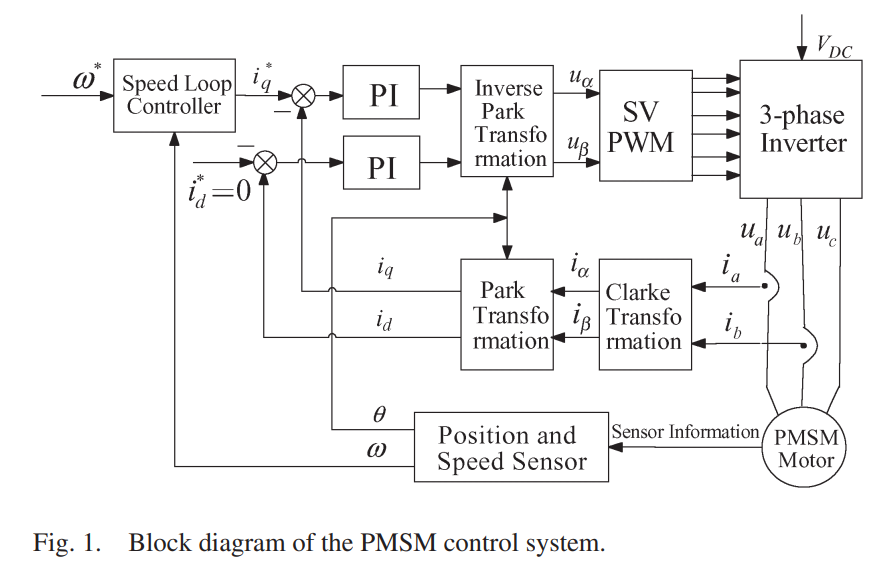
\includegraphics[width=0.7\linewidth]{pmsm_control_block_diag.png}
  \caption{From Liu and Li  ``Speed control for PMSM servo system'', IEEE Transactions on Industrial Electronics, 2012.}
  \label{fig:pmsm-block}
\end{center}
\end{figure}
In the design of the speed controller, it is often assumed that the inner current control loop is sufficiently fast so that the actual current $i_q$ corresponds to the desired current $i_q^*$. The dynamics of the motor can then be simplified and described with the block diagram below. 
\begin{center}
  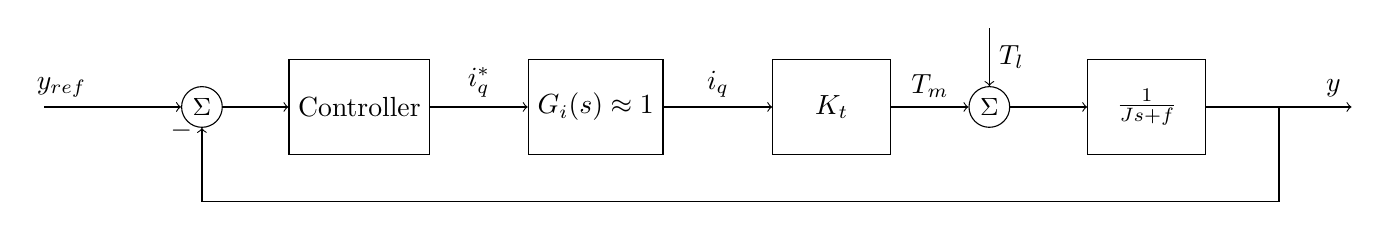
\begin{tikzpicture}[node distance = 2cm, block/.style={draw, minimum height=12mm, minimum width=15mm}]
    \node[coordinate] (input) {};
    \node[circle, draw, inner sep=2pt, right of=input] (sum) {\small $\Sigma$};
    \node[block, right of=sum] (controller) {Controller};
    \node[block, right of=controller, node distance=3cm] (Gi) {$G_i(s) \approx 1$};
    \node[block, right of=Gi, node distance=3cm] (Kt) {$K_t$};
    \node[circle, draw, inner sep=2pt, right of=Kt] (sumdist) {\small $\Sigma$};
    \node[coordinate, right of=sum] (output) {};
    \node[block, right of=sumdist, node distance=2cm] (plant) {$\frac{1}{Js + f}$};
    \node[coordinate, above of=sumdist, node distance=16mm] (dist) {};
    \node[coordinate, right of=plant, node distance=26mm] (output) {};
    
    \draw[->] (input) -- node[above, very near start] {$y_{ref}$} (sum);
    \draw[->] (sum) -- node[] {} (controller);
    \draw[->] (controller) -- node[above,] {$i_q^*$} (Gi);
    \draw[->] (Gi) -- node[above, ] {$i_q$} (Kt);
    \draw[->] (Kt) -- node[above, ] {$T_m$} (sumdist);
    \draw[->] (sumdist) -- node[above,] {$$} (plant);
    \draw[->] (plant) -- node[coordinate] (measure) {} node[above, very near end] {$y$} (output);
    \draw[->] (sumdist) ++ (0,1) -- node[right] {$T_l$} (sumdist);
    \draw[->] (measure) -- ++(0,-1.2) -| node[left, pos=0.98] {$-$} (sum);
  \end{tikzpicture}
\end{center}
In the simplified model, $y$ is the speed, $J$ is the moment of inertia of the motor and load, $f$ is the viscous damping coefficient, $T_m$ is the motor torque and $T_l$ is the load torque. Write $b=\frac{K_t}{J}$, $k=\frac{1}{J}$, and $a=\frac{f}{J}$, which gives the plant model
\begin{equation}
Y(s) = \frac{bI_q(s) + kT_l(s)}{s + a}.
\label{eq:ct-model}
\end{equation}
For a particular motor, which we will consider in this exam, we have $b=\frac{K_t}{J} = \frac{0.7}{1.7\times10^{-4}} \approx  4\times 10^{3}$, $k\approx 5.7\times 10^3$ and $a=\frac{f}{J} = \frac{7.43\times 10^{-5}}{1.74 \times 10^{-4}} \approx 0.4$.  
The chosen sampling period is $h=\unit{10}{\milli\second} = \unit{10^{-2}}{\second}$. The choice is based on a design requirement that the closed-loop system should have a rise-time of \unit{100}{\milli\second}. 
Zero-order hold sampling of the plant gives the following discrete-time model
\begin{equation}
  \underbrace{(\shift - 0.996)}_{A(\shift)} y(k) = \underbrace{40}_{B(q)}i_q(k) + 57\, T_l(k).
  \label{eq:dt-model}
\end{equation}
Including a simplified model of an anti-aliasing filter, the discrete-time system can be represented by the block diagram in figure \ref{fig:block}.
\begin{figure}
\begin{center}
  \begin{tikzpicture}[node distance = 2cm, block/.style={draw, minimum height=10mm, minimum width=15mm}]
    \node[coordinate] (input) {};
    \node[circle, draw, inner sep=2pt, right of=input] (sum) {\small $\Sigma$};
    \node[block, right of=sum] (controller) {Controller};
    \node[block, right of=controller, node distance=3cm] (Kt) {$40$};
    \node[circle, draw, inner sep=2pt, right of=Kt] (sumdist) {\small $\Sigma$};
    \node[coordinate, right of=sum] (output) {};
    \node[block, right of=sumdist, node distance=2cm] (plant) {$\frac{1}{z-0.996}$};
    \node[block, above of=sumdist, node distance=12mm] (kv) {$57$};
    \node[block, below of=plant, node distance=16mm] (aa) {$z^{-1}$};
    \node[coordinate, above of=kv, node distance=16mm] (dist) {};
    \node[coordinate, right of=plant, node distance=26mm] (output) {};
    
    \draw[->] (input) -- node[above, very near start] {$y_{ref}$} (sum);
    \draw[->] (sum) -- node[] {} (controller);
    \draw[->] (controller) -- node[above,] {$i_q$} (Kt);
    \draw[->] (Kt) -- node[above, ] {$ $} (sumdist);
    \draw[->] (sumdist) -- node[above,] {$$} (plant);
    \draw[->] (plant) -- node[coordinate] (measure) {} node[above, very near end] {$y$} (output);
    \draw[->] (kv) ++ (0,1.3) -- node[right] {$T_l$} (kv);
    \draw[->] (kv) -- (sumdist);
    \draw[->] (measure) |- (aa);
    \draw[->] (aa) -| node[left, pos=0.98] {$-$} (sum);
  \end{tikzpicture}
  \caption{Closed-loop system represented in discrete time.}\label{fig:block}
\end{center}
\end{figure}

\begin{exercise}
  Where is the model of the antialiasing filter in the block-diagram of figure \ref{fig:block}? Circle it and explain briefly in 2-4 sentences why this model is used.

\noindent
\fbox{
\bmpl
{\bf Answer:}\\
\vspace*{50mm}
\emp}
\end{exercise}

\begin{exercise}
\abc%
What is the \emph{time-constant} of the plant in the continuous-time model \eqref{eq:ct-model}
\[ Y(s) = \frac{4\times 10^3 I_q(s) + 5.7\times 10^3T_l(s)}{s + a}?\]

\noindent
\fbox{
\bmpl
{\bf Answer}\\
\vspace*{15mm}
\emp}

\abc%
What is the \emph{DC-gain} (static gain) of the pulse-transfer function from $i_q(k)$ to $y(k)$?

\noindent
\fbox{
\bmpl
{\bf Answer:}\\
\vspace*{15mm}
\emp}

\abc%
Below you can see four different unit step-responses. Which one of them corresponds to the system $H(z) = \frac{40}{z-0.996}$? \textbf{Motivate!}
\begin{center}
\begin{tikzpicture}
%\tikzset{plttype/.style={ycomb, thick, mark=*, mark options={red!60!black}}}
\tikzset{plttype/.style={const plot, no marks,  thick}}
  \begin{groupplot} [
    group style={
      group name=timeplot,
      group size=2 by 2,
      xlabels at=edge bottom,
      ylabels at=edge left,
      %horizontal sep=2cm,
      %vertical sep=2cm,
    }, 
    width=8.8cm, height=4cm,
    xlabel={time [s]},
    ylabel={$y(k)$},
    ]
    \nextgroupplot
    \addplot[plttype] table[x=0, y = 4] from \inputtable;% node [coordinate, pos=0.9, pin=-20:{$y(k)$}] {};
    \nextgroupplot
    \addplot[plttype] table[x=0, y = 3] from \inputtable; % node [coordinate, pos=0.9, pin=-20:{$y(k)$}] {};
    \nextgroupplot
    \addplot[plttype] table[x=0, y = 2] from \inputtable; % node [coordinate, pos=0.9, pin=-20:{$y(k)$}] {};
    \nextgroupplot
    \addplot[plttype] table[x=0, y = 1] from \inputtable; % [coordinate, pos=0.9, pin=-20:{$y(k)$}] {};
  \end{groupplot}

\node[red!80!black!90] at ($ (timeplot c1r1.north) + (5mm, -15mm) $) {\huge \rom{1}};
\node[red!80!black!90] at ($ (timeplot c1r2.north) + (5mm, -15mm) $) {\huge \rom{2}};
\node[red!80!black!90] at ($ (timeplot c2r1.north) + (5mm, -15mm) $) {\huge \rom{3}};
\node[red!80!black!90] at ($ (timeplot c2r2.north) + (5mm, -15mm) $) {\huge \rom{4}};

\end{tikzpicture}
\end{center}

\noindent
\fbox{
\bmpl
{\bf Answer and motivation:}\\
\vspace*{70mm}
\emp}
\end{exercise}

\newpage
\begin{exercise}
Using a 2-dof controller (see figure \ref{fig:2dof}), we want to achieve the closed loop system
\begin{equation}
  Y(z) = \frac{B_c(z)}{A_c(z)}Y_{ref}(z) = \frac{(1-0.8)^2}{(z-0.8)^2} Y_{ref}(z),
\end{equation}
from the reference signal to the output. We also want the controller to include an integrator 
\[ F_b(z) = \frac{S(z)}{(z-1)\bar{R}(z)}. \]
\begin{figure}
\begin{center}
\begin{tikzpicture}[node distance=2.6cm, block/.style={rectangle, draw, minimum height=10mm, minimum width=16mm}, sumnode/.style={circle, draw, inner sep=1pt}]

  \node[block] (ffw) {$F_f(z)=\frac{T(z)}{(z-1)\bar{R}(z)}$};
  \node[sumnode, right of=ffw] (sum) {\small $\Sigma$};
  \node[block, right of=controller, node distance=1.4cm] (Kt) {$40$};
  \node[circle, draw, inner sep=2pt, right of=Kt] (sumdist) {\small $\Sigma$};
  \node[block, right of=sumdist, node distance=2cm] (plant) {$\frac{1}{z-0.996}$};
  \node[block, below of=plant, node distance=16mm] (aa) {$z^{-1}$};
  \node[block, below of=Kt, node distance=16mm] (ffb) {$F_b(z)=\frac{S(z)}{(z-1)\bar{R}(z)}$};


  \node[coordinate, left of=ffw, node distance=3cm] (input) {};
  \node[coordinate, above of=sumdist, node distance=1cm] (dist) {};
  \node[block, right of=sumdist, node distance=2cm] (plant) {$\frac{1}{z-0.996}$};
  \node[block, above of=sumdist, node distance=12mm] (kv) {$57$};
  \node[coordinate, above of=kv, node distance=16mm] (dist) {};
  \node[coordinate, right of=plant, node distance=26mm] (output) {};


  \draw[->] (plant) -- node[coordinate] (measure) {} node[above, very near end] {$y$} (output);
  \draw[->] (kv) ++ (0,1.3) -- node[right] {$T_l$} (kv);
  \draw[->] (kv) -- (sumdist);
  \draw[->] (Kt) -- (sumdist);
  

  \draw[->] (input) -- node[above, pos=0.2] {$y_{ref}(k)$} (ffw);
  \draw[->] (ffw) to (sum);
  \draw[->] (sum) -- node[above, ] {$i_q(k)$} (Kt);
  \draw[->] (sumdist) to (plant);
  \draw[->] (measure) |- (aa);
  \draw[->] (aa) to (ffb);
  \draw[->] (ffb) -| node[pos=0.9, right] {$-$} (sum);

\end{tikzpicture}
\caption{A two-degree-of-freedom controller for the PMSM.}\label{fig:2dof}
\end{center}
\end{figure}

\abc%
Determine the \emph{characteristic polynomial} for the closed-loop system from the load disturbance $T_l(k)$ to the output $y(k)$.

\noindent
\fbox{
\bmpl
{\bf Answer:}\\
\vspace*{90mm}
\emp}

\abc%
Write down the \emph{Diophantine equation}. Determine the \emph{degree} of the controller such that all the unknown controller parameters can be uniquely determined from the Diophantine equation.

\noindent
\fbox{
\bmpl
{\bf Answer:}\\
\vspace*{80mm}
\emp}

\abc%
Determine the \emph{degree} of the observer polynomial $A_o(z)$ in $A_{cl}(z)=A_c(z)A_o(z)$. What is the \emph{rule-of-thumb} for choosing the observer poles?

\noindent
\fbox{
\bmpl
{\bf Answer:}\\
\vspace*{50mm}
\emp}


\end{exercise}

\begin{exercise}

[Bonus problem, worth 5p] If the PMSM is part of an industrial installation, it could be subject to noise from the \unit{60}{\hertz} mains hum. What is the \emph{fundamental alias frequency} (the alias frequency below the Nyquist frequency) for the mains hum in the computer-controlled system considered in this exam?
 
\noindent
\fbox{
\bmpl
{\bf Answer:}\\
\vspace*{70mm}
\emp}

\end{exercise}

%\cleardoublepage
%\end{document}

\section*{Solutions}
\setcounter{exerctr}{0} 

\begin{exercise}

The model $z^{-1}$ corresponds to a delay of one sampling period due to the antialiasing filter. Since we use a Bessel-filter as an antialiasing filter, we know that it can be well approximated as a pure delay for low frequencies. When designing the antialiasing filter there is a trade-off between small time delay and attenuation at the Nyquist frequency. Normally the antialiasing filter corresponds to a delay closer to two sampling periods, so the particular filter used here has relative high cutoff-frequency. 

\begin{center}
  \begin{tikzpicture}[node distance = 2cm, block/.style={draw, minimum height=10mm, minimum width=15mm}]
    \node[coordinate] (input) {};
    \node[circle, draw, inner sep=2pt, right of=input] (sum) {\small $\Sigma$};
    \node[block, right of=sum] (controller) {Controller};
    \node[block, right of=controller, node distance=3cm] (Kt) {$40$};
    \node[circle, draw, inner sep=2pt, right of=Kt] (sumdist) {\small $\Sigma$};
    \node[coordinate, right of=sum] (output) {};
    \node[block, right of=sumdist, node distance=2cm] (plant) {$\frac{1}{z-0.996}$};
    \node[block, above of=sumdist, node distance=12mm] (kv) {$57$};
    \node[block, below of=plant, node distance=16mm] (aa) {$z^{-1}$};
    \node[draw,circle, red, thick, inner sep=7mm, below of=plant, node distance=16mm]  {};
    \node[coordinate, above of=kv, node distance=16mm] (dist) {};
    \node[coordinate, right of=plant, node distance=26mm] (output) {};
    
    \draw[->] (input) -- node[above, very near start] {$y_{ref}$} (sum);
    \draw[->] (sum) -- node[] {} (controller);
    \draw[->] (controller) -- node[above,] {$i_q$} (Kt);
    \draw[->] (Kt) -- node[above, ] {$ $} (sumdist);
    \draw[->] (sumdist) -- node[above,] {$$} (plant);
    \draw[->] (plant) -- node[coordinate] (measure) {} node[above, very near end] {$y$} (output);
    \draw[->] (kv) ++ (0,1.3) -- node[right] {$T_l$} (kv);
    \draw[->] (kv) -- (sumdist);
    \draw[->] (measure) |- (aa);
    \draw[->] (aa) -| node[left, pos=0.98] {$-$} (sum);
  \end{tikzpicture}
\end{center}
\end{exercise}

\begin{exercise}
  \abc%
  There are two standard ways of writing a first-order system:
  \[G(s) = \frac{b}{s+a} \quad \text{and} \quad G(s)=\frac{k}{sT+1}.\]
  The time-constant is $T=\frac{1}{a} = \frac{1}{0.4} = \unit{2.5}{\second}$.

  \abc%
  The pulse-transfer function from $i_q$ to $y$ is 
  \[ H(z) = \frac{40}{z-0.996}\]
  and the DC-gain is obtained by evaluating the pulse-transfer function for $z=1$
  \[H(1) = \frac{40}{1-0.996} \approx 9.4\times 10^3.\]

  \abc%
  The correct answer is \textbf{III}. The DC-gain of the system is $H(1)=\frac{1}{1-0.996}\approx 235$, so this is what the unit step response should converge to. So clearly neither I nor II can be the correct response. We know that the time constant is \unit{2.5}{\second} which means that the response should have reached 63\% of 235 after 2.5 seconds, or after 1 second about $0.63\times 235/2.5 \approx 60$. Response IV rises too slowly.  
\end{exercise}

\begin{exercise}
  \abc%
  Write $y(k) = H_l(\shift)T_l(k)$ for the closed-loop system from load disturbance $T_l(k)$ to output $y(k)$. Using Mason's rule we get
  \[ H_l(z) =  \frac{57\frac{1}{z-0.996}}{1 + z^{-1}\frac{40}{z-0.996}\frac{S(z)}{(z-1)\bar{R}(z)}}
            = \frac{57z(z-1)\bar{R}(z)}{z(z-0.996)(z-1)\bar{R}(z) + 40S(z)}. \]

  \abc%
  The Diophantine equation is obtained by setting the characteristic polynomial of the closed-loop system equal to the desired characteristic polynomial. This gives
  \[z(z-0.996)(z-1)\bar{R}(z) + 40S(z) = A_c(z)A_o(z), \]
  where $A_c(z) = (z-0.8)^2$. Write $\deg{\bar{R}} = n_R$. The feedback controller will be
  \[F_b(z) = \frac{s_0z^{n_R+1} + s_1z^{n_R} + \cdots + s_{n_R+1}}{(z-1)(z^{n_R} + r_0z^{n_R-1} + \cdots + r_{n_R})}, \]
  which has $n_R+n_R+1+1=2n_R+2$ unknown parameters. We want the Diophantine equation to be of the same degree, so that we get just enough equations to determine the parameters. The degree of the Diophantine equation is given by the degree of the left-most term which has degree $3+n_R$. We get
  \[2n_R+2 = n_R+3 \quad \Rightarrow \quad n_R = 1.\]
  Written out, the controller we will determine (but not in this exam) is
  \[F_b(z) = \frac{s_0z^2 + s_1z + s_2}{(z-1)(z + r_1)}.\]

  \abc%
  Since the left-hand side has degree $3+n_R=4$, then so must the right-hand side have. We have
  \(A_{cl}(z) = A_c(z)A_o(z) = (z-0.8)^2A_o(z)\), and so $\deg A_o(z) = 2$. The rule-of-thumb is that the observer poles should be chosen to be faster (closer to the origin) than the (other) closed-loop poles. For instance, a dead-beat observer would have poles in the origin, $A_o(z) = z^2$. 
\end{exercise}

\begin{exercise}
  For simplicity,  use Hz instead of rad/s as unit. The sampling period is $h=\unit{10^-2}{\second}$, so the sampling frequency is $f_s = \frac{1}{h} = \unit{100}{\hertz}$, and the Nyquist frequency is $f_N=f_s/2 = \unit{50}{\hertz}$. The fundamental alias $f$ of a frequncy $f_1=\unit{60}{\hertz}$ is given by the formula
  \[ f = | \big( (f_1 + f_N) \mod f_s \big) - f_N | = | \big( (60 + 50) \mod 100 \big) - 50 | = \unit{40}{\hertz}.\]
  You can also arrive at the correct result by noting how the frequency \unit{60}{\hertz} is \emph{folded} about the Nyquist frequency \unit{50}{\hertz}
  \begin{center}
    \begin{tikzpicture}
      \draw[->] (-1,0) --  node[below, pos=1] {Hz} (10,0);
      \draw[dashed, red] (5,-0.1) --(5,1);
      \node at (5,-0.4) {\small $50$};
      \draw[black,->] (6,0) --(6,1);
      \node at (6,-0.4) {\small $60$};
      \draw[blue,->] (4,0) --(4,1);
      \node at (4,-0.4) {\small $40$};
      \node at (0,-0.4) {\small $0$};
    \end{tikzpicture}
  \end{center}
\end{exercise}
\end{document}
